% Built from the official competition Overleaf template, retrieved 2026-09-28.
\documentclass[sigconf]{acmart}
% =============================================================================
% Template setup — participants normally do not edit this file.
% Author content belongs in main.tex; citations belong in main.bib.
% \documentclass lives in main.tex so Overleaf does not treat this file as root.
% =============================================================================

% --- Competition / non-ACM-submission friendly rights metadata -------------
\setcopyright{none}
\settopmatter{printacmref=false}
\acmConference[Kaggle Competition]{Filament Segmentation Challenge}{2026}{\href{https://www.kaggle.com/competitions/filament-segmentation-2026}{kaggle.com/competitions/filament-segmentation-2026}}
\acmBooktitle{Competition Report}
\acmDOI{}
\acmISBN{}

% --- Author guidance text --------------------------------------------------
% \guide{...} is gray italic while \guideStyletrue; omitted from the PDF if false.
% Flip the switch in main.tex after % =============================================================================
% Template setup — participants normally do not edit this file.
% Author content belongs in main.tex; citations belong in main.bib.
% \documentclass lives in main.tex so Overleaf does not treat this file as root.
% =============================================================================

% --- Competition / non-ACM-submission friendly rights metadata -------------
\setcopyright{none}
\settopmatter{printacmref=false}
\acmConference[Kaggle Competition]{Filament Segmentation Challenge}{2026}{\href{https://www.kaggle.com/competitions/filament-segmentation-2026}{kaggle.com/competitions/filament-segmentation-2026}}
\acmBooktitle{Competition Report}
\acmDOI{}
\acmISBN{}

% --- Author guidance text --------------------------------------------------
% \guide{...} is gray italic while \guideStyletrue; omitted from the PDF if false.
% Flip the switch in main.tex after % =============================================================================
% Template setup — participants normally do not edit this file.
% Author content belongs in main.tex; citations belong in main.bib.
% \documentclass lives in main.tex so Overleaf does not treat this file as root.
% =============================================================================

% --- Competition / non-ACM-submission friendly rights metadata -------------
\setcopyright{none}
\settopmatter{printacmref=false}
\acmConference[Kaggle Competition]{Filament Segmentation Challenge}{2026}{\href{https://www.kaggle.com/competitions/filament-segmentation-2026}{kaggle.com/competitions/filament-segmentation-2026}}
\acmBooktitle{Competition Report}
\acmDOI{}
\acmISBN{}

% --- Author guidance text --------------------------------------------------
% \guide{...} is gray italic while \guideStyletrue; omitted from the PDF if false.
% Flip the switch in main.tex after \input{preamble}.
%
% Do not use \guide{...} for \email{...}.
\usepackage{xcolor}
\newif\ifguideStyle
\guideStyletrue
\newcommand{\guide}[1]{%
  \ifguideStyle
    {\color{gray!65}\itshape #1}%
  \fi
}

% --- Math ------------------------------------------------------------------
% Do NOT load amssymb (or amsfonts): acmart already loads newtxmath, which
% defines the same symbols (e.g. \Bbbk) and causes a conflict on Overleaf.
% amsmath is already provided by acmart; mathtools extends it.
\usepackage{mathtools}

% --- Figures ---------------------------------------------------------------
% graphicx is already loaded by acmart
\usepackage{subcaption}

% --- Tables ----------------------------------------------------------------
% booktabs is already loaded by acmart
\usepackage{tabularx}
\usepackage{multirow}

% --- Bibliography style is set in main.tex (ACM-Reference-Format) ----------
.
%
% Do not use \guide{...} for \email{...}.
\usepackage{xcolor}
\newif\ifguideStyle
\guideStyletrue
\newcommand{\guide}[1]{%
  \ifguideStyle
    {\color{gray!65}\itshape #1}%
  \fi
}

% --- Math ------------------------------------------------------------------
% Do NOT load amssymb (or amsfonts): acmart already loads newtxmath, which
% defines the same symbols (e.g. \Bbbk) and causes a conflict on Overleaf.
% amsmath is already provided by acmart; mathtools extends it.
\usepackage{mathtools}

% --- Figures ---------------------------------------------------------------
% graphicx is already loaded by acmart
\usepackage{subcaption}

% --- Tables ----------------------------------------------------------------
% booktabs is already loaded by acmart
\usepackage{tabularx}
\usepackage{multirow}

% --- Bibliography style is set in main.tex (ACM-Reference-Format) ----------
.
%
% Do not use \guide{...} for \email{...}.
\usepackage{xcolor}
\newif\ifguideStyle
\guideStyletrue
\newcommand{\guide}[1]{%
  \ifguideStyle
    {\color{gray!65}\itshape #1}%
  \fi
}

% --- Math ------------------------------------------------------------------
% Do NOT load amssymb (or amsfonts): acmart already loads newtxmath, which
% defines the same symbols (e.g. \Bbbk) and causes a conflict on Overleaf.
% amsmath is already provided by acmart; mathtools extends it.
\usepackage{mathtools}

% --- Figures ---------------------------------------------------------------
% graphicx is already loaded by acmart
\usepackage{subcaption}

% --- Tables ----------------------------------------------------------------
% booktabs is already loaded by acmart
\usepackage{tabularx}
\usepackage{multirow}

% --- Bibliography style is set in main.tex (ACM-Reference-Format) ----------

\usepackage{balance}
\guideStylefalse
\settopmatter{printfolios=true}
\begin{document}
\title[Global Context, Native Detail]{Global Context, Native Detail: Validated Solar Filament Segmentation on a Single GPU}
\subtitle{A Solution to the Solar Filament Segmentation Challenge 2026}
\author{Anon Tokyo}
\email{pufanzhang1@gmail.com}
\renewcommand{\shortauthors}{Anon Tokyo}

\begin{abstract}
This report describes our solution to the Solar Filament Segmentation Challenge~2026, a Kaggle competition on automatic segmentation of solar filaments in GONG H-$\alpha$ observations.
We combine a ConvNeXt U-Net at 1536-pixel resolution with an instance-conditioned refiner operating on native-resolution crops. The design separates global detection from local mask correction and rejection, while preserving thin structures during instance grouping. Five folds group nearby observations and retain all annotations of each image together. Under the organizers' evaluator, the fixed refined recipe achieves out-of-fold panoptic quality (PQ) of 0.4427, versus 0.4287 for coarse proposals. The gain remains positive on the four confirmation folds: $+0.0149$ PQ, with a paired temporal-group bootstrap 95\% interval of $[0.0118,0.0182]$. Public submissions score 0.38, so we distinguish validated local improvements from unconfirmed test gains. We document both successful refinements and rejected alternatives, quantify the remaining small-instance recall deficit, and release an auditable inference and evaluation pipeline. Memory-mapped supervision, asynchronous transfers and compact mask decoding make this workflow practical on one 32\,GB GPU.
\end{abstract}
\maketitle

\section{Introduction}
This report goes over the details of our submitted solution to the Solar Filament Segmentation Challenge~2026 \cite{filament-segmentation-2026}. The challenge, launched on July~10,~2026, is organized by the Earth-Space AI Research (ESAIR) Lab\footnote{\href{https://www.esairlab.com/home}{www.esairlab.com/}}. This challenge utilizes the MAGFiLO dataset for evaluation of the segmentation algorithms \cite{ahmadzadeh2024dataset}.
We contribute native-crop refinement, consistent multi-annotator evaluation and engineering for controlled single-GPU experiments. Cross-fold confirmation takes priority over isolated development scores.

\section{Methodology}\label{sec:methodology}
\subsection{Data and grouped validation}
The official training split contains 707 distinct $2048\!\times\!2048$ grayscale images, 1,154 annotator--image entries and 8,199 filament instances; the test split contains 180 images. Only the provided segmentation masks supervise our task-specific training. ImageNet-pretrained encoders supply generic visual initialization. Auxiliary supplied spines, classes and bounding boxes are not training targets; candidate geometry is derived from masks.

We freeze five folds containing 142/143/141/140/141 images. All annotators of an observation remain together. Chronologically adjacent images with gaps at most 72 hours are grouped within an initial 14-day window; exact duplicate image hashes are also grouped. This produces 331 groups. Date and station identifiers support partitioning and auditing, not model inputs. The split reduces temporal dependence but cannot prove complete physical independence. Fold~0 is the development fold; folds~1--4 confirm the selected post-processing recipe. The manifest and checkpoints carry matching SHA256 provenance.

\subsection{Global semantic proposals}
A ConvNeXt-Tiny encoder~\cite{convnext} with a U-Net decoder~\cite{unet} predicts foreground and boundary logits. The five decoder stages have 256, 128, 64, 32 and 16 channels. Normalized grayscale is replicated into the three encoder input channels. We first train at 1024 pixels for 30 epochs, then fine-tune at 1536 pixels for 24 epochs, retaining checkpoints selected by instance-level PQ. Each sample selects one annotator uniformly and constructs its foreground union and instance-boundary target; we do not merge different annotators into one evaluation truth.

The loss is foreground binary cross-entropy (BCE) plus soft Dice, with $0.2$ times a boundary BCE term (positive weight 3). Augmentation combines right-angle rotations, flips, photometric perturbations and occasional mild blur or noise. AdamW uses decoder learning rates $3\!\times\!10^{-4}$ then $10^{-4}$, encoder rates one fifth as large, weight decay 0.01, warmup/cosine decay and EMA decay 0.99. The effective baseline batch size is four. BF16 arithmetic and gradient clipping stabilize training.

Inference averages logits from the identity, horizontal flip and vertical flip views. Probabilities are resized to the native grid and thresholded at 0.5. An 8-pixel dilation defines connected \emph{groups} of nearby foreground fragments, but each output mask retains only original foreground pixels: dilation does not thicken the submitted filament. Proposals smaller than 64 native pixels are removed. Equal-weight fold ensembles operate on probability maps before instance extraction.

\begin{figure*}[t]
\centering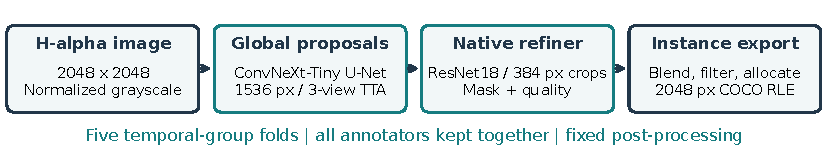
\includegraphics[width=\textwidth]{figures/pipeline.pdf}
\caption{End-to-end pipeline. Grouped training and the official per-annotator evaluation apply to both learned stages. Global probability ensembling precedes extraction; all refiners then see the same candidate masks.}
\Description{Four stages: grayscale solar image, global semantic proposals, native local refinement, and non-overlapping instance export.}
\label{fig:pipeline}
\end{figure*}

\subsection{Native instance refinement and rejection}
The second U-Net uses a ResNet18 encoder~\cite{resnet}, a four-channel input (three normalized image channels plus the candidate mask), one mask output and a pooled quality head. Native $384\!\times\!384$ crops preserve detail without resizing small filaments down to a full-disk training grid. Training uses proposals from the corresponding outer training fold; 25\% of samples instead start from perturbed training masks. Random annotator selection preserves annotation diversity. Poor proposals supply empty-target negatives, and morphology/translation perturbations reduce dependence on exact training proposals. The refiner is trained for 12 epochs with 6,000 sampled crops per epoch, batch 48, AdamW at $3\!\times\!10^{-4}$ and EMA. Its loss is BCE + Dice + $0.1$ quality BCE. The quality target indicates a nonempty crop with proposal--annotation IoU above 0.3; it is a learned rejection score, not a calibrated probability of an official match.

Inference expands each proposal box by 48 pixels and processes large regions using overlapping native crops with stride 256. Positive Hann weights fuse crop probabilities; crop quality scores are averaged. We retain quality $\geq0.5$, average the refined probability with a Gaussian-smoothed proposal ($\sigma=2$ pixels), threshold at 0.5 and require 64 pixels. Confidence-ordered pixel allocation makes instances mutually exclusive before COCO RLE export. The full recipe includes mask refinement, quality filtering and a changed area threshold; its gain is not attributed solely to boundary correction.

The released test ensemble uses five Tiny fold models (weight 0.1 each), two V2-Base models excluding folds 0 and 1 (weight 0.25 each), and five equal-weight refiners on identical proposals. V2 uses 40/18 training epochs at 1024/1536 pixels. Extraction settings remain fixed. A separate all-data Tiny/refiner pair uses the fixed 30/24/12-epoch schedule and supplies no held-out evidence. The release manifest records the submitted CSV and checkpoint hashes.

\section{Evaluation}\label{sec:evaluation}
\subsection{Protocol and uncertainty}
We reproduce the organizers' self-evaluation notebook: IoU $>0.5$ defines a match, the same image prediction is evaluated separately for each annotator, and counts are accumulated globally:
\begin{equation}
\mathrm{PQ}=\frac{\sum_{(g,p)\in TP}\mathrm{IoU}(g,p)}{|TP|+\tfrac12|FP|+\tfrac12|FN|}.
\end{equation}
PQ combines recognition quality (RQ) and matched-mask quality (SQ)~\cite{panoptic}. A strict one-to-one matching diagnostic accompanies the official count-based implementation. For the refined OOF result, strict PQ is 0.4426 versus official 0.4427, indicating negligible sensitivity to this distinction.

Table~\ref{tab:oof} compares the frozen refinement recipe against coarse predictions with a 256-pixel minimum area. Every validation image is predicted by models excluding its fold. This estimates the single-fold recipe, \emph{not} a held-out five-model test ensemble. We resample temporal groups 5,000 times, keeping all annotators and paired predictions together. Intervals describe uncertainty conditional on the fitted models; they do not account for repeated development-fold model selection.

\begin{table}[t]
\centering\small
\caption{Frozen-recipe OOF results. Fold~0 is development; folds~1--4 are confirmation. Pooled PQ is computed from counts, not averaged fold scores.}
\label{tab:oof}
\begin{tabular}{lrrr}\toprule
Held-out fold & Coarse PQ & Refined PQ & $\Delta$ PQ\\\midrule
0 & 0.4318 & 0.4414 & +0.0096\\
1 & 0.4134 & 0.4319 & +0.0186\\
2 & 0.4361 & 0.4501 & +0.0139\\
3 & 0.4280 & 0.4421 & +0.0142\\
4 & 0.4348 & 0.4478 & +0.0130\\\midrule
Pooled 1--4 & 0.4280 & 0.4430 & +0.0149\\
Pooled 0--4 & 0.4287 & \textbf{0.4427} & +0.0139\\\bottomrule
\end{tabular}
\end{table}

\subsection{What improved, and what did not}
Refinement improves all five folds. Across all annotation entries, false positives fall from 3,234 to 2,627 ($18.8\%$), while true positives fall slightly from 5,305 to 5,244. SQ changes from 0.6763 to 0.6783 and RQ from 0.6339 to 0.6526. Thus the principal benefit is better instance precision, with a measurable recall trade-off. Pooled refined PQ has a 95\% interval $[0.4327,0.4523]$; the paired gain interval is $[0.0111,0.0168]$. Confirmation-only evidence remains positive (Table~\ref{tab:oof}).

We tested increasingly expensive or permissive alternatives (Table~\ref{tab:ablation}). Native 2048-pixel global training and eight-view TTA did not beat the 1536-pixel baseline. Hysteresis grouping produced only a small development gain. Extra geometry/intensity scoring and disconnected-component cleanup moved refined PQ by less than 0.001 and were not promoted. The initial sparse-loss Mask2Former run collapsed; a dense-loss retry reached checkpoint-selection PQ 0.2756 but remained below the semantic baseline. These are budget-limited results, not evidence against the architecture generally.

ConvNeXt-V2-Base~\cite{convnextv2} added modest complementary signal. Equal architecture mixing after refinement improved fold~0 from 0.4414 to 0.4477 and fold~1 from 0.4319 to 0.4360. However, the fold~1 gain interval $[-0.0032,0.0104]$ crosses zero. Single-fold, five-fold, mixed-backbone and all-data submissions all display public PQ 0.38. We therefore do not claim a demonstrated public improvement from ensembling or a reliable private-score forecast.

Calibrated Mask R-CNN reaches 0.4035, or 0.4254 after refinement. Adding isolated refined detections reaches 0.4431; the gain interval spans $-0.0009$ to $0.0047$. Quality-loss weight 0.5, component balancing, sampling by annotation count and native-tile training yield 0.4408, 0.4416, 0.4393 and 0.4397 respectively. None justifies changing the recipe.

\begin{table}[t]
\centering\small
\caption{Development-fold ablations. Comparisons within each block share the indicated reference; these are not independent test estimates.}
\label{tab:ablation}
\begin{tabular}{lr}\toprule
Coarse proposal variant & Fold~0 PQ\\\midrule
1536 px, three-view flips (reference) & \textbf{0.4318}\\
Native 2048 px & 0.4262\\
Eight-view dihedral TTA & 0.4316\\
1536 + 2048 probability ensemble & 0.4311\\
Hysteresis grouping & 0.4327\\\midrule
Refined variant & Fold~0 PQ\\\midrule
Frozen refinement (reference) & 0.4414\\
Geometry + refiner quality selection & 0.4421\\
Small-island cleanup & 0.4416\\
Morphological closing, radius 6 & 0.4398\\
Tiny + V2-Base, refined & 0.4477\\\bottomrule
\end{tabular}
\end{table}

\begin{figure*}[t]
\centering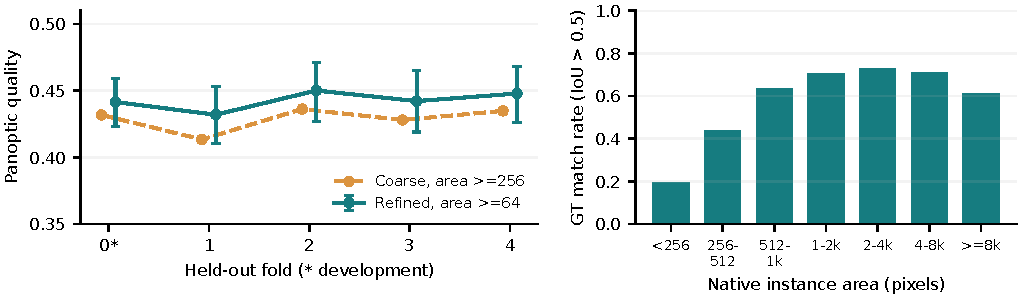
\includegraphics[width=\textwidth]{figures/validation.pdf}
\caption{Left: refinement improves each fold; error bars are temporal-group bootstrap 95\% intervals for refined PQ. Right: small ground-truth instances remain difficult; matching uses IoU $>0.5$ at native resolution.}
\Description{Five-fold coarse versus refined PQ with uncertainty, and ground-truth match rates grouped by instance area.}
\label{fig:validation}
\end{figure*}

\subsection{Morphology and remaining errors}
Only 493 of 1,131 annotated instances with area 256--512 pixels are matched ($43.6\%$), compared with $70.6\%$ at 1024--2048 pixels and $72.9\%$ at 2048--4096 pixels. Higher global resolution alone did not fix this gap. Candidate discrimination and small, faint filament recall remain more promising than uniform mask dilation, which damaged PQ.

Figure~\ref{fig:distributions} reports best-prediction IoU and Dice for \emph{every} annotated filament, including misses as zeros, rather than showing only successful matches. We also count one-to-many and many-to-one overlap relations per annotator--image using any nonzero intersection; these diagnostics differ from the stricter PQ matching criterion. Figure~\ref{fig:examples} illustrates both failures and accurate delineation. Its examples are selected from held-out predictions by proximity to prespecified IoU levels, not presented as a random performance sample.

\begin{figure*}[t]
\centering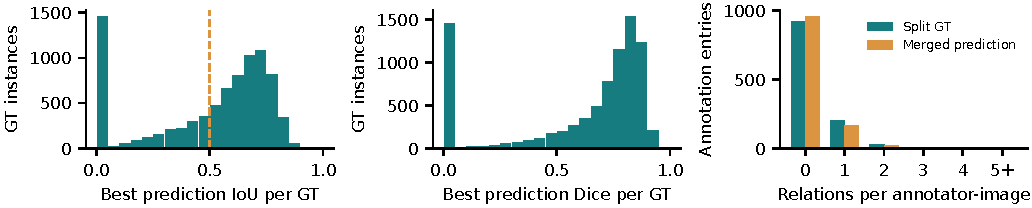
\includegraphics[width=\textwidth]{figures/distributions.pdf}
\caption{OOF quality distributions include all 8,199 annotated instances. The dashed line marks the PQ match threshold. Split/merge counts use nonzero overlap and retain separate annotator entries; full numerical arrays accompany the report.}
\Description{Histograms of best IoU and Dice per ground-truth instance, plus distributions of split and merge counts.}
\label{fig:distributions}
\end{figure*}

\begin{figure*}[t]
\centering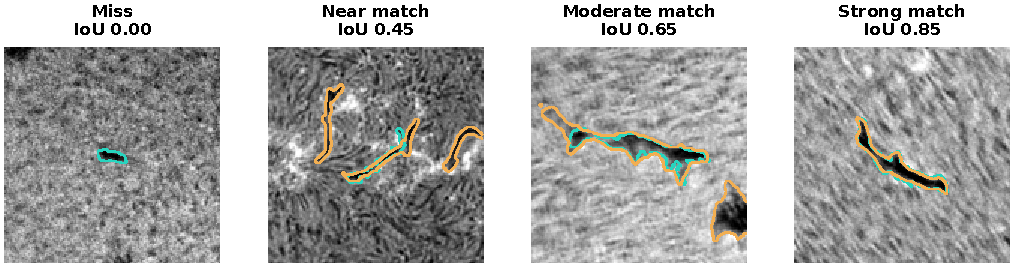
\includegraphics[width=\textwidth]{figures/qualitative.pdf}
\caption{Native held-out crops with annotated instance in teal and predictions in amber. Columns target best-IoU levels 0, 0.45, 0.65 and 0.85, with distinct images and areas 256--6,000 pixels. A miss and a near match accompany successful cases; image IDs, folds and crop coordinates are provided with the figures.}
\Description{Four grayscale solar crops with corresponding ground-truth and predicted contour overlays, spanning missed through well-matched filaments.}
\label{fig:examples}
\end{figure*}

\section{Engineering and reproducibility}
Experiments use PyTorch~2.8, Python~3.12 and CUDA~12.8 on an RTX~5090 (32\,GB); the final host provides 16 vCPUs and approximately 90\,GB usable RAM. Packed/memory-mapped targets avoid repeated full-resolution mask decoding. Persistent workers, pinned memory, a separate CUDA transfer stream, channels-last convolution, fused AdamW and grouped EMA updates reduce training stalls. CPU validation overlaps subsequent GPU training, with checkpoint provenance preserved. CPU thread counts are bounded for the migrated host.

For Mask R-CNN, uint8 targets reduce mask storage fourfold; disabling cuDNN searches for variable ROI batches yields approximately 26-second steady 1024-pixel epochs. Compact ROI decoding preserves exact RLE output on six image/resolution checks. Its sampled 1536-pixel CPU microbenchmark falls from 0.57--0.58 to 0.005--0.007 seconds per image; this is not an end-to-end semantic-pipeline speedup.

Run records preserve configuration, manifest hash, metrics and model state. Submission checks enforce native shape, valid RLE, unique IDs, test coverage and disjoint masks. Fold checks reject invalid validation reuse. Released inference fixes CUDA algorithm selection for repeatable exports. Our \href{https://github.com/zhang0894/Solar-Filament-Segmentation-Challenge-2026-by-Anon-Tokyo}{public repository} provides versioned dependencies, the complete notebook, experiment tables, inference configuration, checkpoint checksums and regeneration commands. Development choices and negative results remain visible.

\section{Limitations and next steps}
The public score remains below local PQ; temporal grouping and conditional bootstrap intervals cannot eliminate distribution uncertainty or selection bias. Refiner proposals are generated on their outer training fold, so their error distribution may be easier than held-out proposals; an inner-OOF proposal curriculum would address this at additional compute cost. Multiple annotators disagree about both presence and shape, and the system cannot satisfy every annotation simultaneously. We do not infer a universal accuracy ceiling from this disagreement. Future work should prioritize hard-negative discrimination and small-instance recall, with cross-fold confirmation before adding model complexity.

\section{Acknowledgment}\label{sec:acknowledgment}
The organization of the Filament Segmentation Challenge 2026 is partially supported by the U.S. National Science Foundation (NSF) under Grant No. 2209912 and 2433781, directorate for Computer and Information Science and Engineering (CSE), and Office of Advanced Cyberinfrastructure (OAC), and Grant No. 2511630, AST Division Of Astronomical Sciences and MPS Directorate for Mathematical and Physical Sciences.

The Filament Segmentation Challenge 2026 is sponsored by the U.S. National Science Foundation (NSF) National Solar Observatory (NSO).

This work utilizes GONG data obtained by the NSO Integrated Synoptic Program, managed by the National Solar Observatory, which is operated by the Association of Universities for Research in Astronomy (AURA), Inc. under a cooperative agreement with the National Science Foundation and with contribution from the National Oceanic and Atmospheric Administration. The GONG network of instruments is hosted by the Big Bear Solar Observatory, High Altitude Observatory, Learmonth Solar Observatory, Udaipur Solar Observatory, Instituto de Astrofísica de Canarias, and Cerro Tololo Interamerican Observatory.

\balance
\bibliographystyle{ACM-Reference-Format}
\bibliography{main}
\end{document}
